\documentclass[12pt]{article}
\usepackage[utf8]{inputenc}
\usepackage{amsmath}
\usepackage{amssymb}
\usepackage{hyperref}
\usepackage{geometry}
\usepackage{graphicx}
\geometry{a4paper, margin=1in}

\title{Assignment 02 Q2: Ant Colony Optimization (ACO) Simulation}
\author{Computational Intelligence}
\date{\today}

\begin{document}

\maketitle

\section{Introduction}
This report provides detail of the Ant Colony Optimization (ACO) simulation implemented for Q2. The simulation visualizes how a swarm of agents (ants) navigates a complex, continuous 3D fitness landscape to locate global minima (valleys) using pheromones and distance heuristic as desirability.

\section{Problem Formulation}
The goal of the simulation is to solve a continuous optimization problem in a 2D search space.

\begin{itemize}
    \item \textbf{Objective Function}: Find the global minimum of the landscape $f(x, y)$.
    \item \textbf{Landscape Construction}: The terrain is generated using a combination of multiple Gaussian valleys and a sinusoidal noise layer.
    \begin{equation}
        f(x, y) = 1.0 - \sum_{i=1}^{N} d_i \cdot \exp\left(-\frac{(x-x_i)^2 + (y-y_i)^2}{2w_i^2}\right) + \text{noise}(x, y)
    \end{equation}
    Where $(x_i, y_i)$ are valley centers, $d_i$ is depth, and $w_i$ is width.
    \item \textbf{Search Space}: A continuous 2D plane ($1000 \times 800$ units), discretized into a grid for pheromone tracking and visualization.
\end{itemize}

\section{Concept behind Simulation}
The simulation is inspired by the foraging behavior of real ant colonies.

\subsection{Pheromone Update Rule}
Pheromone levels are updated at each iteration through a combination of evaporation and pheromone deposition, as defined by the rule:
\begin{equation}
    \tau_{t+1} = (1 - \rho)\tau_t + \Delta \tau_t
\end{equation}

\begin{itemize}
    \item \textbf{Deposition ($\Delta \tau$)}: Ants deposit pheromone based on the fitness of their current location. Areas with lower fitness values (deeper valleys) receive higher pheromone concentrations.
    \begin{equation}
        \Delta \tau \propto \frac{Q}{f(x, y) - f_{\min} + \epsilon}
    \end{equation}
    \item \textbf{Evaporation ($\rho$)}: A constant fraction of the pheromone is removed at each step to prevent premature convergence and encourage exploration.
\end{itemize}

\subsection{Distance Heuristic ($\eta$)}
Agents are also attracted by their local information of where the direction of the nearest minima is through neighbourhood cells. In this simulation, desirability is formulated as the inverse of the local terrain height, guiding ants towards downward slopes even in the absence of pheromones.

\subsection{Probabilistic Movement}
The probability of an ant moving to a neighbouring cell $j$ is determined by the computing transition probabilities:
\begin{equation}
    P_{ij} = \frac{[\tau_j]^\alpha \cdot [\eta_j]^\beta}{\sum [\tau_k]^\alpha \cdot [\eta_k]^\beta}
\end{equation}
Where:
\begin{itemize}
    \item $\alpha$: Importance of pheromone (exploitation).
    \item $\beta$: Importance of local heuristic (exploration/greediness).
\end{itemize}

\section{Implementation Details}
The simulation is built using the \textbf{Processing} framework.

\subsection{Discretization}
While Ant Colony Optimization is traditionally applied to discrete combinatorial problems (e.g., TSP), this implementation applies it to a continuous fitness landscape by employing discretization. The $1000 \times 800$ space is mapped to a grid where each $5 \times 5$ cell acts as a node in a graph. This approach was chosen to provide a clear idea of the entire landscape's promising regions.

\subsection{Algorithmic Specifics}
\begin{itemize}
    \item \textbf{Core Logic}: The simulation runs an iterative loop where ants evaluate 8-direction neighborhoods, move probabilistically, deposit pheromones, and the global pheromone map undergoes evaporation.
    \item \textbf{Convergence Tracking}: A real-time graph tracks the ``Global Best'' fitness over iterations, demonstrating the algorithm's ability to converge on the deepest valleys.
    \item \textbf{Interactivity}: Users can adjust parameters in real-time using keyboard controls:
    \begin{itemize}
        \item \textbf{[A/a]}: Increase/decrease $\alpha$ (pheromone influence)
        \item \textbf{[B/b]}: Increase/decrease $\beta$ (heuristic influence)
        \item \textbf{[E/e]}: Increase/decrease $\rho$ (evaporation rate)
        \item \textbf{[P/p]}: Increase/decrease ant population (±10)
        \item \textbf{[SPACE]}: Pause/resume simulation
        \item \textbf{[R]}: Reset simulation with new random ant positions
        \item \textbf{[Click]}: Add new valley at mouse position
        \item \textbf{[S]}: Save screenshot
    \end{itemize}
\end{itemize}


\subsection{Visual Design}
The simulation employs the following visual cues to enhance understanding:
\begin{itemize}
    \item \textbf{Terrain Gradient}: The terrain transitions from flat lands (brown) to deep valleys (green), providing an intuitive topographic visualization where the intensity of the color indicates the depth.
    \item \textbf{Contour Lines}: Dark lines delineate elevation levels for easier terrain interpretation
    \item \textbf{Pheromone Trails}: Yellow-to-red gradient indicates trail intensity (darker red = higher traffic)
    \item \textbf{Ant Representation}: White-outlined black dots for individual agents
    \item \textbf{Global Best Indicator}: Pulsing circle marks the current best-known location
\end{itemize}

\newpage

\section{Simulation Visualization}
The following figure showcases the ant colony's behavior as it converges toward the global minima. The colored trails represent pheromone concentrations, where darker reds indicate high-traffic areas and successful optimization.

\begin{figure}[h!]
    \centering
    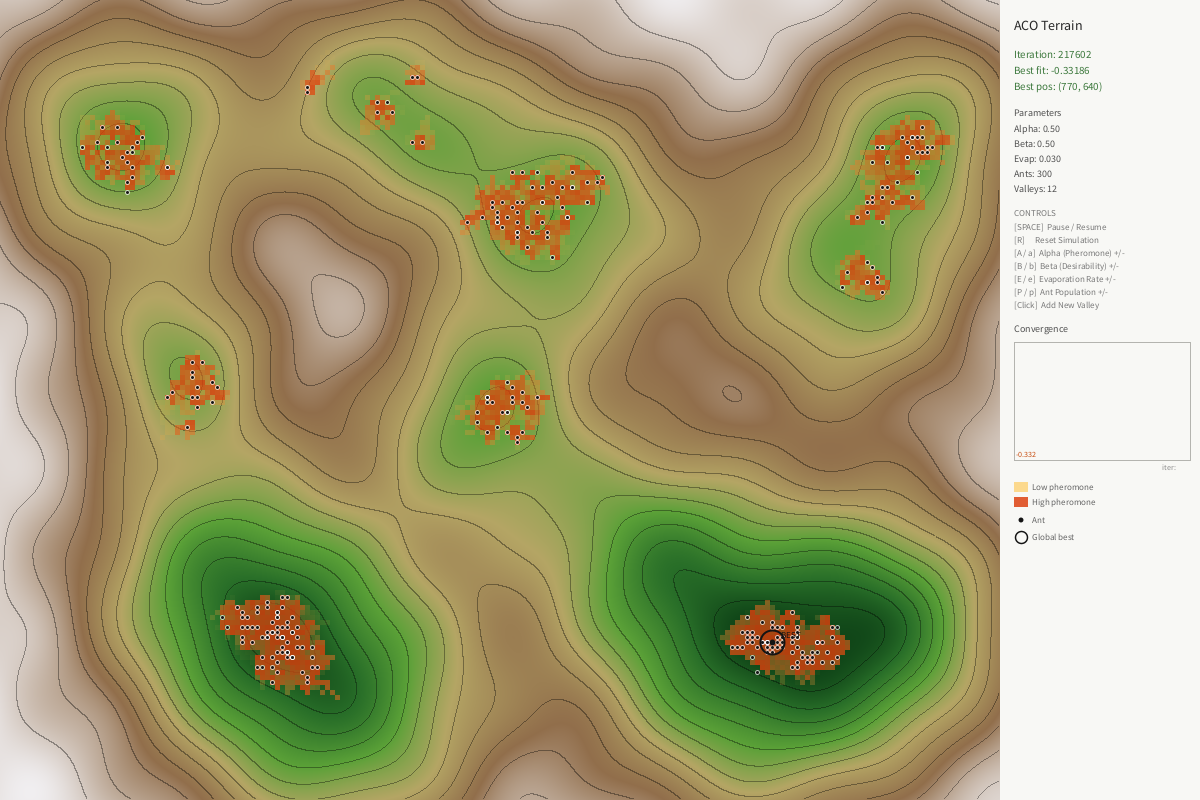
\includegraphics[width=0.8\textwidth]{screenshot.png}
    \caption{Ant colony exploring and converging on the discretised fitness landscape. Majority of ants have converged to a minima.}
    \label{fig:simulation}
\end{figure}

\section{Simulation Video}
The following link demonstrates the simulation in action: \\
\textbf{Video Link:} \url{https://www.youtube.com/watch?v=4SkZhGsgaXk}

\end{document}

